\subsection{Module Graph}\label{app:module-detail}

\subsubsection{Containment Decay}

\begin{table}[ht]
\centering
\caption{Module-level containment decay by module depth. At depth~$1$ ($13$ top-level packages), $97.5\%$ of import edges stay within the same package; by depth~$4$, containment has fallen to~$8.8\%$.}
\label{tab:module-containment}
\begin{tabular}{crrr}
\toprule
Depth $k$ & Groups & Containment & $\Delta$ (pp) \\
\midrule
$1$ & $13$      & $97.5\%$  & ---     \\
$2$ & $99$      & $60.2\%$  & $-37.3$ \\
$3$ & $1{,}481$ & $34.1\%$  & $-26.1$ \\
$4$ & $5{,}641$ & $8.8\%$   & $-25.3$ \\
$5$ & $7{,}434$ & $0.8\%$   & $-8.0$  \\
\bottomrule
\end{tabular}
\end{table}

At depth~$1$, the $13$ top-level packages (\module{Mathlib}, \module{Batteries}, \module{Init}, etc.) contain $97.5\%$ of all import edges. The steepest single drop occurs at depth~$1 \to 2$ ($-37.3$ pp), when packages split into their subdirectories. The $60.2\%$ containment at depth~$2$ is consistent with the $61.4\%$ intra-directory rate reported in \S\ref{sec:cross-namespace}.\footnote{The small discrepancy ($60.2\%$ vs.\ $61.4\%$) reflects a difference in edge counts between our import parser and the \texttt{importGraph} tool.} By depth~$4$---the modal depth of modules---containment has fallen to $8.8\%$, and by depth~$5$ it is negligible.

\subsubsection{Cross-Directory Heatmaps}\label{app:module-heatmaps}

\begin{figure}[H]
\centering
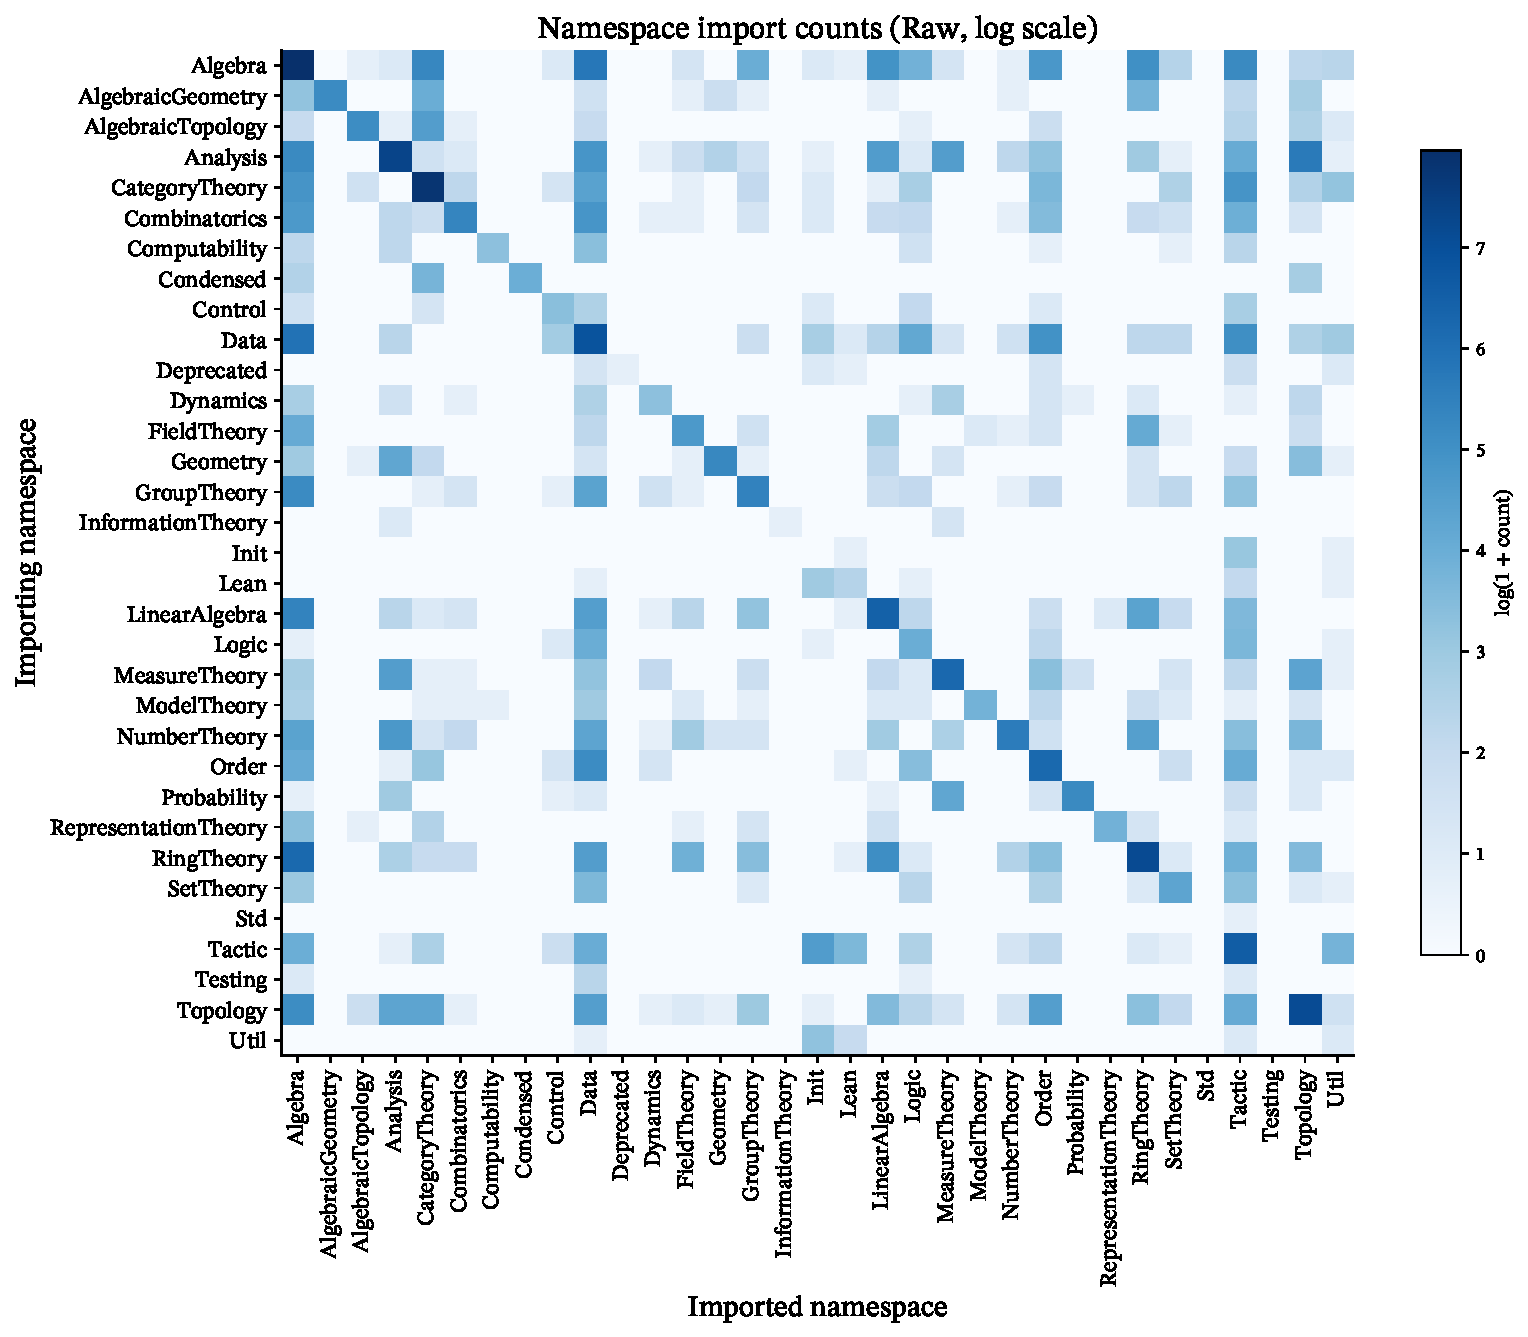
\includegraphics[width=\textwidth]{figures/namespace_heatmap_raw.pdf}
\caption{Import counts between top-level directories (log scale) for $G_{\mathrm{module}}$. Each cell $(i, j)$ counts edges from directory~$i$ (row) to directory~$j$ (column); the diagonal captures intra-directory imports. Off-diagonal bright cells reveal cross-directory dependencies that violate the cognitive classification of~$T$.}
\label{fig:namespace-heatmap-raw}
\end{figure}

\begin{figure}[H]
\centering
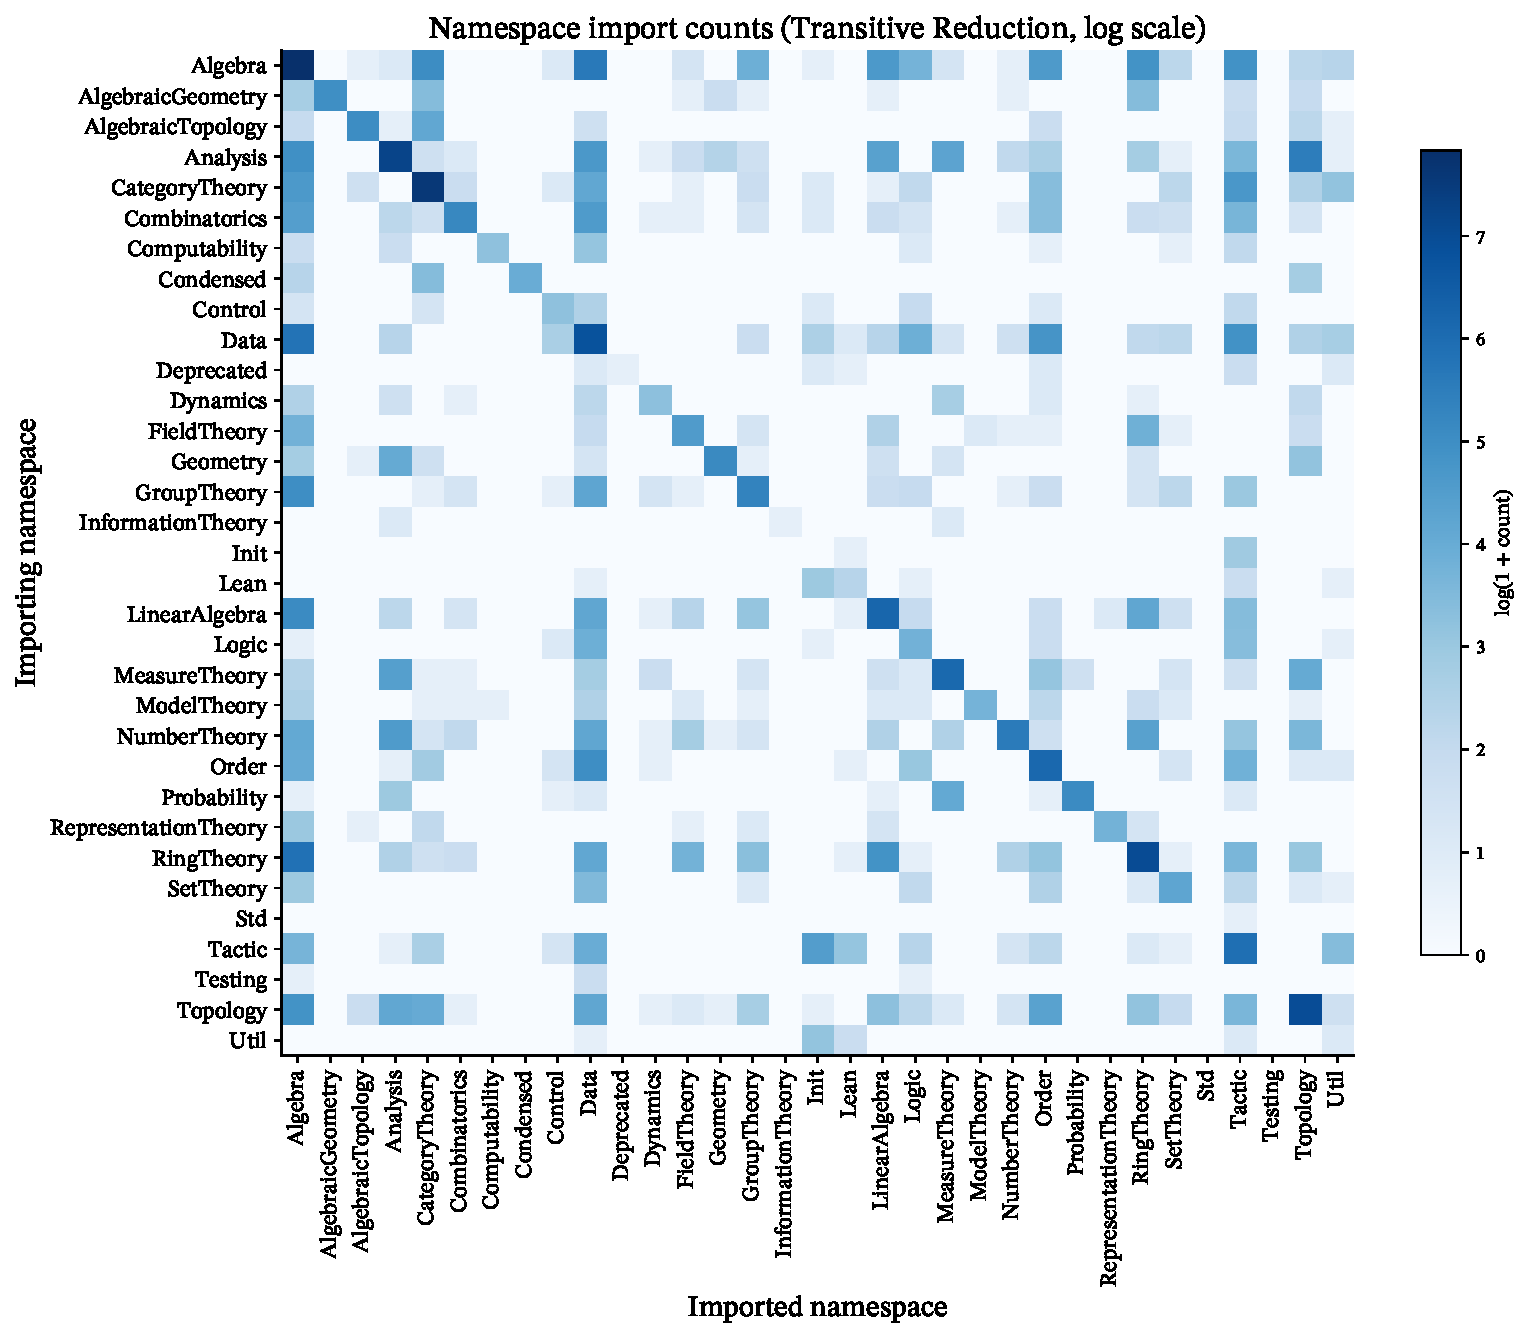
\includegraphics[width=\textwidth]{figures/namespace_heatmap_tr.pdf}
\caption{Import counts between top-level directories (log scale) for $G_{\mathrm{module}}^{-}$ (transitive reduction). Compared to the raw graph (Figure~\ref{fig:namespace-heatmap-raw}), the transitive reduction removes redundant edges while preserving the essential dependency skeleton. The most prominent off-diagonal entries include \module{RingTheory}$\,\to\,$\module{Algebra} and the bidirectional coupling between \module{Algebra} and \module{Data}.}
\label{fig:namespace-heatmap-tr}
\end{figure}

\subsubsection{Extended Analysis}\label{app:module-analysis}

\noindent \textit{1. The tension between logical precision and cognitive management.} \\
The divergence between the raw module graph $G_{\mathrm{module}}$ and its transitive reduction $G_{\mathrm{module}}^{-}$ quantifies the human cost of organizing logic. The 17.5\% edge redundancy (\S\ref{sec:transitive-reduction}) is not merely inefficiency; it represents the \textit{cognitive API} of the library.\oliver{SHAKE: (1) ``cognitive API'' $\to$ ``development ergonomics layer.'' (2) ``maintain mental models'' $\to$ ``ease refactoring and future extensibility.'' (3) Note post-shake on 17.5\%.} Developers import entire theories (umbrella modules) to maintain mental models of the library, sacrificing logical minimality for usability.

Dependency for compilation follows the strict logical requirements of the type checker, ensuring that the build system avoids cycles and minimizes checking time. In contrast, dependency for discovery serves the human prover and the automation: it brings tactics, notation, and type class instances into scope, populating the context for search and elaboration.\oliver{SHAKE: This ``dependency for discovery'' framing partially aligns with Oliver's point---tactics, notation, and typeclass instances are exactly the development-ergonomic reasons for keeping imports. But reframe away from ``cognitive'' framing toward ``engineering/development workflow'' framing.} We argue that the 17.5\% redundancy observed in \module{Mathlib} is not an inefficiency but a structural feature that creates robustness against refactoring and simplifies the user interface.\oliver{SHAKE: (1) Note post-shake. (2) The ``robustness against refactoring'' part aligns well with Oliver's framing---emphasize this over ``cognitive API.'' (3) Should also note that shake intentionally preserves some of these imports, suggesting the Mathlib community agrees they serve a structural purpose.} Optimizing solely for the transitive reduction would likely degrade the interactive experience, suggesting that future proof assistants could benefit from explicitly modeling these two layers separately: a minimal graph for the build system and a rich, redundant graph for the user.

\medskip
\noindent \textit{2. The architectural source of compilation bottlenecks.} \\
The layer-width profile (\S\ref{sec:dag-depth}) reveals a distinct \textit{funnel topology}: a massive leaf layer ($>1,400$ modules) resting on a deep, narrow foundation. This extreme verticality (DAG depth~$153$; \S\ref{sec:dag-depth}) contrasts sharply with the flatter citation graphs of informal mathematics. While this depth ensures rigorous consistency, it creates significant structural fragility: changes in the narrow ``waist'' of the funnel (high-betweenness modules) trigger massive recompilation cascades.\oliver{MODULE: The ``narrow waist'' / ``compilation bottleneck'' is exactly what the module system (Nov 2025) was designed to address. Oliver explicitly mentioned this. Note: (1) the module system allows private imports to reduce transitive visibility, directly shrinking the recompilation cascade; (2) the ``federated tiers'' speculation in the next paragraph is essentially what the module system implements at the language level.} This identifies a critical scalability challenge: as libraries grow, the depth of the dependency chain becomes a liability that may require aggressive modularization or distinct compilation units.

Moreover, this topology imposes a distinct evolutionary pressure on the library's development. Unlike informal mathematics, where foundational texts are static references, the modules in \module{Mathlib}'s ``theoretical waist'' remain mutable code. The depth of 153 layers implies that the maintenance cost of a lemma is strictly a function of its topological depth: a change in the narrow waist invalidates the verification of thousands of downstream results. One possible trajectory is that monolithic libraries will eventually hit a \textit{critical depth threshold} where the cost of coherence checks exceeds the capacity for rapid iteration. If so, future architectures may need to break this funnel into \textit{federated tiers}---effectively freezing the foundational layers into pre-compiled artifacts---to decouple the logical necessity of depth from the operational necessity of build speed.\oliver{MODULE: This ``federated tiers'' conjecture is essentially what the module system does: private imports create compilation boundaries that decouple layers. Reframe as noting the module system as an existing response, not a hypothetical future.} This remains a conjecture unsupported by longitudinal data; whether the current depth of $153$ layers is approaching such a threshold, or is comfortably sustainable, cannot be determined from a single snapshot.

Our analysis captures a single snapshot (commit \texttt{534cf0b}). Whether these structural properties are stable or evolving---and whether the 17.5\% redundancy rate and DAG depth of~$153$ are increasing, stable, or approaching a critical threshold---remains an open question that longitudinal analysis across \module{Mathlib} versions must address.\oliver{SHAKE: Note post-shake on 17.5\%.}

\medskip
\noindent \textit{3. Centrality as a proxy for maintenance roles.} \\
We propose that the centrality measures computed in \S\ref{sec:centrality} can be interpreted as distinct maintenance signals.
\begin{itemize}
    \item \textit{In-degree} identifies the \textit{vocabulary} of the library (utilities used locally).
    \item \textit{PageRank} identifies the \textit{axiomatic core} (the deep dependencies that underpin the truth of the system).
    \item \textit{Betweenness} identifies \textit{structural bridges} (modules that connect disparate mathematical subfields).
\end{itemize}
Refactoring a high-betweenness module is riskier than refactoring a high in-degree module, as the former disrupts the connective tissue between theories. From an engineering perspective, the PageRank and betweenness rankings (Table~\ref{tab:centrality}) offer a principled priority ordering for compilation optimization and CI resource allocation: modifications to high-centrality modules may warrant broader downstream testing.

\medskip
\noindent \textit{Hypothesis: The Curated Small-World.} \\
We hypothesize that successful formal libraries naturally evolve into \textit{curated small-world networks}. Unlike social networks which grow via preferential attachment, \module{Mathlib} grows via \textit{semantic attachment}: new modules cluster tightly within top-level directories (high local clustering), while bridge modules with high betweenness maintain global connectivity.

The fact that 100\% of modules belong to a single weakly connected component provides empirical evidence for the structural unification of mathematical theories within \module{Mathlib}. The density of inter-directory edges (37.1\%, \S\ref{sec:cross-namespace}) functions as a system of high-betweenness shortcuts that prevent the library from fracturing into isolated ``theory islands.'' Our analysis of targeted node removal (Table~\ref{tab:robustness}) demonstrates that this connectivity is remarkably resilient: over 99\% of modules remain in the giant component even after the removal of the five most central hubs.

The curated small-world is the form in which the tension between $T$ and $G_{\mathrm{module}}$ reaches dynamic equilibrium---but this equilibrium is not static. The module tree $T$ actively shapes $G_{\mathrm{module}}$: developers import along the cognitive contours of $T$, producing the 62.9\% intra-directory concentration and the directional redundancy identified in \S\ref{sec:transitive-reduction}. Simultaneously, $G_{\mathrm{module}}$ reshapes $T$: the 37.1\% of edges that cross directory boundaries exert pressure on the cognitive classification, and \module{Mathlib}'s ongoing directory reorganizations---such as the gradual absorption of \module{RingTheory} into \module{Algebra}---are precisely the points where logical necessity forces cognitive categories to yield. Neither $T$ alone nor $G_{\mathrm{module}}$ alone determines the architecture; each continuously remakes the other.

This mutual determination also governs the library's evolution. The accumulation of DAG depth ($153$; \S\ref{sec:dag-depth}), cross-directory density (37.1\%), and hub concentration represents the growing tension between logical structure and cognitive organization. In this sense, formalization does not dissolve the human organization of mathematics, nor does it simply reveal where that organization must yield. It initiates a feedback loop: the formal product reshapes the cognitive framework that produced it, which in turn reshapes the next generation of formal products.

\label{sec:structural-analysis}
\subsubsection{Degree Distribution}
\label{sec:degree-distribution}
\label{sec:sa-degree}

In $G_{\mathrm{module}}$, the out-degree $\deg^{+}(m) = |\mathrm{imports}(m)|$: it counts the number of modules that $m$ directly imports. The in-degree $\deg^{-}(m)$ counts how many other modules depend on~$m$.
Structurally, in-degree measures how foundational a module is---how many others build upon it---while out-degree measures how much of the library a module assembles. A high in-degree module is \emph{infrastructure}; a high out-degree module is an \emph{integrator}.

\begin{table}[H]
\centering
\caption{Degree statistics for $G_{\mathrm{module}}$ and its transitive reduction~$G_{\mathrm{module}}^{-}$.}
\label{tab:degree-stats}
\begin{tabular}{lrrrr}
\toprule
& \multicolumn{2}{c}{$G_{\mathrm{module}}$} & \multicolumn{2}{c}{$G_{\mathrm{module}}^{-}$} \\
\cmidrule(lr){2-3} \cmidrule(lr){4-5}
& In-degree & Out-degree & In-degree & Out-degree \\
\midrule
Mean   & $3.12$ & $3.12$ & $2.57$ & $2.57$ \\
Median & $2$    & $3$    & $1$    & $2$    \\
Std    & $4.69$ & $4.12$ & $3.91$ & $1.83$ \\
Max    & $167$  & $315$  & $151$  & $70$   \\
\bottomrule
\end{tabular}
\end{table}

The module with the highest in-degree in both graphs is \module{Mathlib.Init} ($\deg^{-} = 167$ in $G_{\mathrm{module}}$, $151$ in $G_{\mathrm{module}}^{-}$), the foundational module that most files depend on. Other high in-degree modules include \module{Tactic.Common} ($74$), \module{Analysis.Normed.Group.Basic} ($57$), and \module{Algebra.Ring.Defs} ($42$). The highest out-degree belongs to \module{Mathlib.Tactic} ($315$ in $G_{\mathrm{module}}$), which serves as an umbrella file aggregating tactic imports; transitive reduction reduces this to~$60$.

We plot the degree distributions on log--log axes (Figure~\ref{fig:degree-distribution}).

\begin{figure}[H]
\centering

\includegraphics[width=\textwidth]{figures/degree_distribution.pdf}
\caption{In-degree (blue) and out-degree (orange) distributions on log--log axes for $G_{\mathrm{module}}$ (left) and $G_{\mathrm{module}}^{-}$ (right). Dashed lines show power-law references $k^{-\gamma}$. Two features are visually salient: (i)~the in-degree distributions are nearly identical across the two panels, confirming that transitive reduction barely affects how many modules depend on a given file; (ii)~the out-degree tail contracts sharply under transitive reduction (maximum dropping from $315$ to $70$), reflecting the removal of redundant umbrella imports.}
\label{fig:degree-distribution}
\end{figure}

\noindent\textbf{Note.}
Both degree distributions are heavy-tailed but do not cleanly fit a power law. The out-degree distribution, in particular, becomes much more concentrated after transitive reduction (maximum dropping from $315$ to $70$, standard deviation from $4.12$ to $1.83$), indicating that many high-out-degree imports are transitively redundant.
In contrast, the in-degree distribution is barely affected by transitive reduction (maximum: $167 \to 151$; standard deviation: $4.69 \to 3.91$). This asymmetry has a structural explanation: redundant edges arise primarily from developers importing umbrella modules---an act that inflates the importer's out-degree without changing the importee's in-degree. The cognitive redundancy identified in \S\ref{sec:transitive-reduction} is \emph{directional}: it lives in the ``I depend on others'' direction, not the ``others depend on me'' direction.
This directional asymmetry connects to the tree $T$: developers inflate their out-degree by importing umbrella modules that aggregate entire sub-hierarchies---effectively borrowing $T$'s cognitive categories as navigational shortcuts. The redundancy is not random; it follows the contours of~$T$.\oliver{SHAKE: ``cognitive categories as navigational shortcuts'' should be reframed as ``organizational structure for development ergonomics.'' The imports follow $T$ because developers want easy access to related theory for future extensions, not primarily for navigation.}

\subsubsection{DAG Depth and Layered Structure}
\label{sec:dag-depth}

All sources (modules with no incoming edges) sit at level~$0$, while the unique sink \module{Tactic.Linter.DirectoryDependency} sits at level~$153$.

The depth of $G_{\mathrm{module}}$ is $153$, attained by a path from \module{NumberTheory.LSeries.PrimesInAP} (a leaf-level number theory result) down to \module{Tactic.Linter.DirectoryDependency} (a low-level linter utility). This path traverses number theory, special functions, measure theory, topology, order theory, logic, and tactic infrastructure---reflecting the deep dependency chain required to formalize analytic number theory.

$G_{\mathrm{module}}$ has $1{,}433$ source modules (files that no other \module{Mathlib} file imports) and exactly $1$~sink (\module{Tactic.Linter.DirectoryDependency}, the unique module with no imports within Mathlib). The topological levels partition $\mathcal{M}$ into $154$ layers, with a maximum layer width of $1{,}433$ (the source layer) and a median width of~$25$.

Notably, the layer-width profiles of $G_{\mathrm{module}}$ and $G_{\mathrm{module}}^{-}$ are nearly identical: the number of layers, the position of the peak, and the overall funnel shape are preserved under transitive reduction. This means that the vertical structure of the dependency chain reflects genuine logical necessity rather than cognitive redundancy---the 17.5\% redundant edges identified in \S\ref{sec:transitive-reduction} add lateral shortcuts within layers but do not alter the depth of the graph.\oliver{SHAKE: Note post-shake on 17.5\%.}

A secondary peak is visible near level~$126$, where approximately $59$ modules concentrate---roughly $6$ to $15$ times the width of surrounding layers. This anomaly warrants further investigation; it may reflect a layer of tactic infrastructure or a mathematical theory that branches into many parallel lemmas at a specific depth.

\begin{figure}[H]
\centering

\includegraphics[width=\textwidth]{figures/dag_structure.pdf}
\caption{DAG width by topological layer for $G_{\mathrm{module}}$ (top) and $G_{\mathrm{module}}^{-}$ (bottom). The distributions share a characteristic funnel shape: a sharp peak at level~$0$ (over $1{,}400$ leaf modules), a rapid decay through the first $20$ layers, a long tail extending to level~$153$, and a secondary peak near level~$126$. The near-identical profiles confirm that the funnel topology arises from logical necessity, not from redundant imports.}
\label{fig:dag-structure}
\end{figure}

\noindent\textbf{Note.}
The layer-width profile has a characteristic ``funnel'' shape: very wide at the top (many independent leaf files), narrowing through the middle layers (where mathematical theories converge), and tapering to a single sink at the bottom. This shape reflects the fact that advanced mathematics is built on a narrow foundation of shared definitions and tactics. This narrow waist also has engineering consequences: any change to a module in the bottleneck layers propagates upward through a large fraction of the library, creating recompilation cascades whose cost grows with the depth of the funnel.\oliver{MODULE: Mention the module system here as an existing engineering response to this narrow-waist problem.}

\noindent\textbf{Module depth and import symmetry.}
\label{rem:import-depth-symmetry}
The DAG depth of~$153$ layers describes the topological extent of the dependency chain. A different notion of depth---the \emph{module depth}, i.e., the number of dot-separated components of a module's fully qualified name---describes how deeply a module sits in the naming hierarchy~$T$. Module depth is concentrated: $55.7\%$ of modules have depth~$4$ (e.g., \module{Mathlib.Data.Nat.Basic}), with a mean of~$4.22$. Import edges exhibit near-perfect depth symmetry: $55.4\%$ connect modules at the same naming depth, $23.3\%$ point from deeper to shallower, and $21.3\%$ from shallower to deeper (mean difference~$+0.03$). Only~$1.3\%$ of imports target modules at depth~$\le 2$. Developers import \emph{laterally}---peer to peer within the same naming stratum---rather than vertically across naming layers. As we shall see in \S\ref{sec:cross_level}, this symmetry contrasts sharply with the declaration-level dependency graph, where $37.6\%$ of edges flow from deeper to shallower namespaces and the mean depth difference rises to~$+0.36$: the module graph compresses and hides the strong infrastructure pull that the declaration graph reveals.

\subsubsection{Centrality}
\label{sec:centrality}
\label{sec:sa-centrality}

We compare three centrality measures---in-degree, PageRank, and betweenness (Definition~\ref{def:pagerank}--\ref{def:betweenness})---to identify the most structurally important modules.

\begin{table}[H]
\centering
\caption{Top~10 modules by in-degree, PageRank, and betweenness centrality in $G_{\mathrm{module}}$.}
\label{tab:centrality}
\small
\begin{tabular}{rlrlrl}
\toprule
\multicolumn{2}{c}{In-degree} & \multicolumn{2}{c}{PageRank} & \multicolumn{2}{c}{Betweenness} \\
\cmidrule(lr){1-2} \cmidrule(lr){3-4} \cmidrule(lr){5-6}
$\deg^{-}$ & Module & PR & Module & $c_B$ & Module \\
\midrule
167 & \module{Init}               & .0435 & \module{Init}              & .0113 & \module{Tactic.Common} \\
 74 & \module{Tactic.Common}      & .0316 & \module{Tactic.Linter.Header} & .0037 & \module{Init} \\
 57 & \module{AN.Group.Basic}     & .0285 & \module{Tactic.Linter.DD}  & .0032 & \module{LA.Span.Basic} \\
 45 & \module{Util.CompileInd.}   & .0058 & \module{Tactic.TypeStar}   & .0030 & \module{AN.Module.FD} \\
 42 & \module{Algebra.Ring.Defs}  & .0048 & \module{Algebra.Group.Defs} & .0024 & \module{Analysis.RCLike} \\
 39 & \module{ABO.Finset.Basic}   & .0038 & \module{Tactic.Basic}      & .0021 & \module{AS.Limits.Basic} \\
 38 & \module{Algebra.Field.Defs} & .0037 & \module{CT.Equivalence}    & .0020 & \module{AS.Limits.Normed} \\
 38 & \module{Algebra.Group.Basic}& .0033 & \module{Logic.Function}    & .0019 & \module{LA.Determinant} \\
 37 & \module{Tactic.Fin.Attr}    & .0030 & \module{Logic.Equiv.Defs}  & .0019 & \module{CT.Category.Basic} \\
 37 & \module{Tactic.TypeStar}    & .0030 & \module{CT.Opposites}      & .0017 & \module{Tactic.NormNum} \\
\bottomrule
\end{tabular}
\end{table}

\noindent
\textit{Abbreviations:} AN = \module{Analysis.Normed}, LA = \module{LinearAlgebra}, CT = \module{CategoryTheory},\\
ABO = \module{Algebra.BigOperators.Group}, AS = \module{Analysis.SpecificLimits},\\
FD = \module{FiniteDimension}, DD = \module{DirectoryDependency}, CompileInd.\ = \module{CompileInductive}, Fin.\ = \module{Finiteness}.
We compare in-degree, PageRank, and betweenness pairwise in Figures~\ref{fig:centrality-indeg-pr}--\ref{fig:centrality-betw-pr}. Out-degree is omitted from this comparison because it measures a module's role as an \emph{importer}---how many prerequisites it gathers---rather than its structural position within the network. Moreover, as shown in \S\ref{sec:degree-distribution}, high out-degree values largely reflect redundant umbrella imports and collapse under transitive reduction, making out-degree a poor proxy for structural importance.

\begin{figure}[H]
\centering
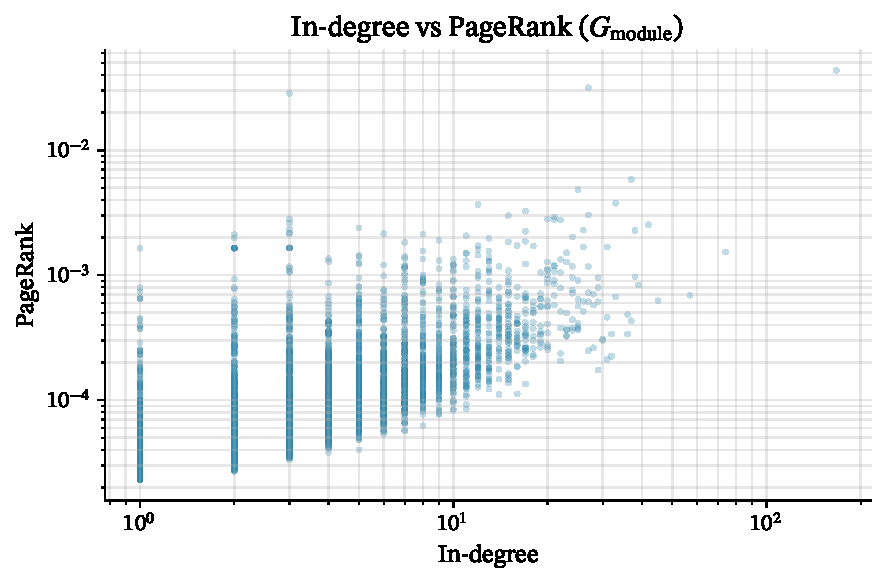
\includegraphics[width=\textwidth]{figures/module_centrality_indeg_pr.pdf}
\caption{In-degree vs.\ PageRank in $G_{\mathrm{module}}$. Each point is one module. If the two measures were equivalent, points would cluster along a diagonal; the wide scatter confirms they capture distinct structural roles.}
\label{fig:centrality-indeg-pr}
\end{figure}

\begin{figure}[H]
\centering

\includegraphics[width=\textwidth]{figures/module_centrality_indeg_betw.pdf}
\caption{In-degree vs.\ betweenness centrality in $G_{\mathrm{module}}$. Modules with high betweenness but moderate in-degree serve as structural bridges between otherwise disconnected regions of the import graph.}
\label{fig:centrality-indeg-betw}
\end{figure}

\begin{figure}[H]
\centering

\includegraphics[width=\textwidth]{figures/module_centrality_betw_pr.pdf}
\caption{Betweenness vs.\ PageRank in $G_{\mathrm{module}}$. The three-way divergence visible in Tables~\ref{tab:centrality} is not confined to the top extremes but pervades the entire distribution.}
\label{fig:centrality-betw-pr}
\end{figure}

The three rankings largely differ: the only module appearing in all three top-20 lists is \module{Mathlib.Init}. This divergence is not a technical detail---it is one of our central findings. It demonstrates that \emph{importance} in a formal mathematical library is irreducibly multidimensional: a module can be heavily used (high in-degree) without being foundational (high PageRank), and foundational without being a bridge (high betweenness). No single centrality measure captures the full structural role of a module; the three measures together define a taxonomy that we develop further in \S\ref{sec:module_conclusion}.

In particular, high-betweenness modules acquire their bridging role precisely by connecting regions of $G_{\mathrm{module}}$ that the tree $T$ separates. The top betweenness modules in Table~\ref{tab:centrality} typically sit at the boundary between top-level directories: they are the points where the logical structure of mathematics forces a passage across $T$'s cognitive borders.

In-degree identifies the most frequently \emph{imported} modules (foundational definitions and commonly used tactics). PageRank, which propagates importance along dependency chains, promotes modules deep in the import hierarchy such as \module{Tactic.Linter.Header} and low-level logic utilities. Betweenness centrality highlights \emph{bottleneck} modules through which many shortest paths pass, favoring files like \module{LinearAlgebra.Span.Basic} and \module{Analysis.Normed.Module.FiniteDimension} that bridge otherwise distant parts of the library.

\subsubsection{Community Structure}
\label{sec:module-community}
\label{sec:sa-community}

We apply Louvain community detection (\S\ref{sec:prelim-community}) to the undirected projection of $G_{\mathrm{module}}$ ($7{,}563$ nodes, $23{,}570$ edges).

\begin{table}[ht]
\centering
\caption{Community detection summary for $G_{\mathrm{module}}$.}
\label{tab:module-community-summary}
\begin{tabular}{lr}
\toprule
Metric & Value \\
\midrule
Number of communities & $16$ \\
Modularity & $0.6395$ \\
Communities with ${>}1{,}000$ nodes & $3$ \\
Communities with ${>}100$ nodes & $9$ \\
\bottomrule
\end{tabular}
\end{table}

The modularity of $0.64$ is the highest among the three levels---substantially above the declaration level ($0.48$) and the namespace level ($0.28$). This reflects the fact that modules are the unit at which human organization is most direct: developers place related files in the same directory, creating dense within-directory import clusters that Louvain readily detects.

\begin{table}[ht]
\centering
\caption{The nine major communities of $G_{\mathrm{module}}$ (Louvain, ${>}100$ nodes), with dominant top-level directories.}
\label{tab:module-communities}
\small
\begin{tabular}{rrl}
\toprule
ID & Size & Dominant directories \\
\midrule
2  & $1{,}445$ & \module{RingTheory} (531), \module{Algebra} (377), \module{LinearAlgebra} (253) \\
7  & $1{,}398$ & \module{CategoryTheory} (893), \module{Algebra} (147), \module{Topology} (92) \\
3  & $1{,}366$ & \module{Algebra} (382), \module{Data} (297), \module{Tactic} (295) \\
1  & $948$     & \module{Analysis} (533), \module{Topology} (124), \module{Geometry} (97) \\
5  & $668$     & \module{Data} (184), \module{Order} (181), \module{Topology} (58) \\
6  & $504$     & \module{MeasureTheory} (232), \module{Probability} (112), \module{Analysis} (88) \\
4  & $455$     & \module{Topology} (233), \module{Analysis} (78), \module{Data} (41) \\
0  & $343$     & \module{Algebra} (111), \module{GroupTheory} (99), \module{Combinatorics} (52) \\
8  & $207$     & \module{Algebra} (102), \module{CategoryTheory} (38) \\
\bottomrule
\end{tabular}
\end{table}

The communities map recognizably onto mathematical domains. \module{CategoryTheory} again dominates a single community ($64\%$ of Community~$7$), mirroring the exceptional autonomy observed at the declaration level (\S\ref{sec:thm-community}). The NMI between Louvain communities and top-level directories is $0.42$ (ARI~$= 0.28$)---higher than the declaration-level NMI of $0.34$ (\S\ref{sec:thm-community}). The stronger alignment reflects the fact that modules, unlike declarations, are explicitly organized into a directory tree; the import graph inherits much of that tree structure.
\begin{figure}[H]
\centering
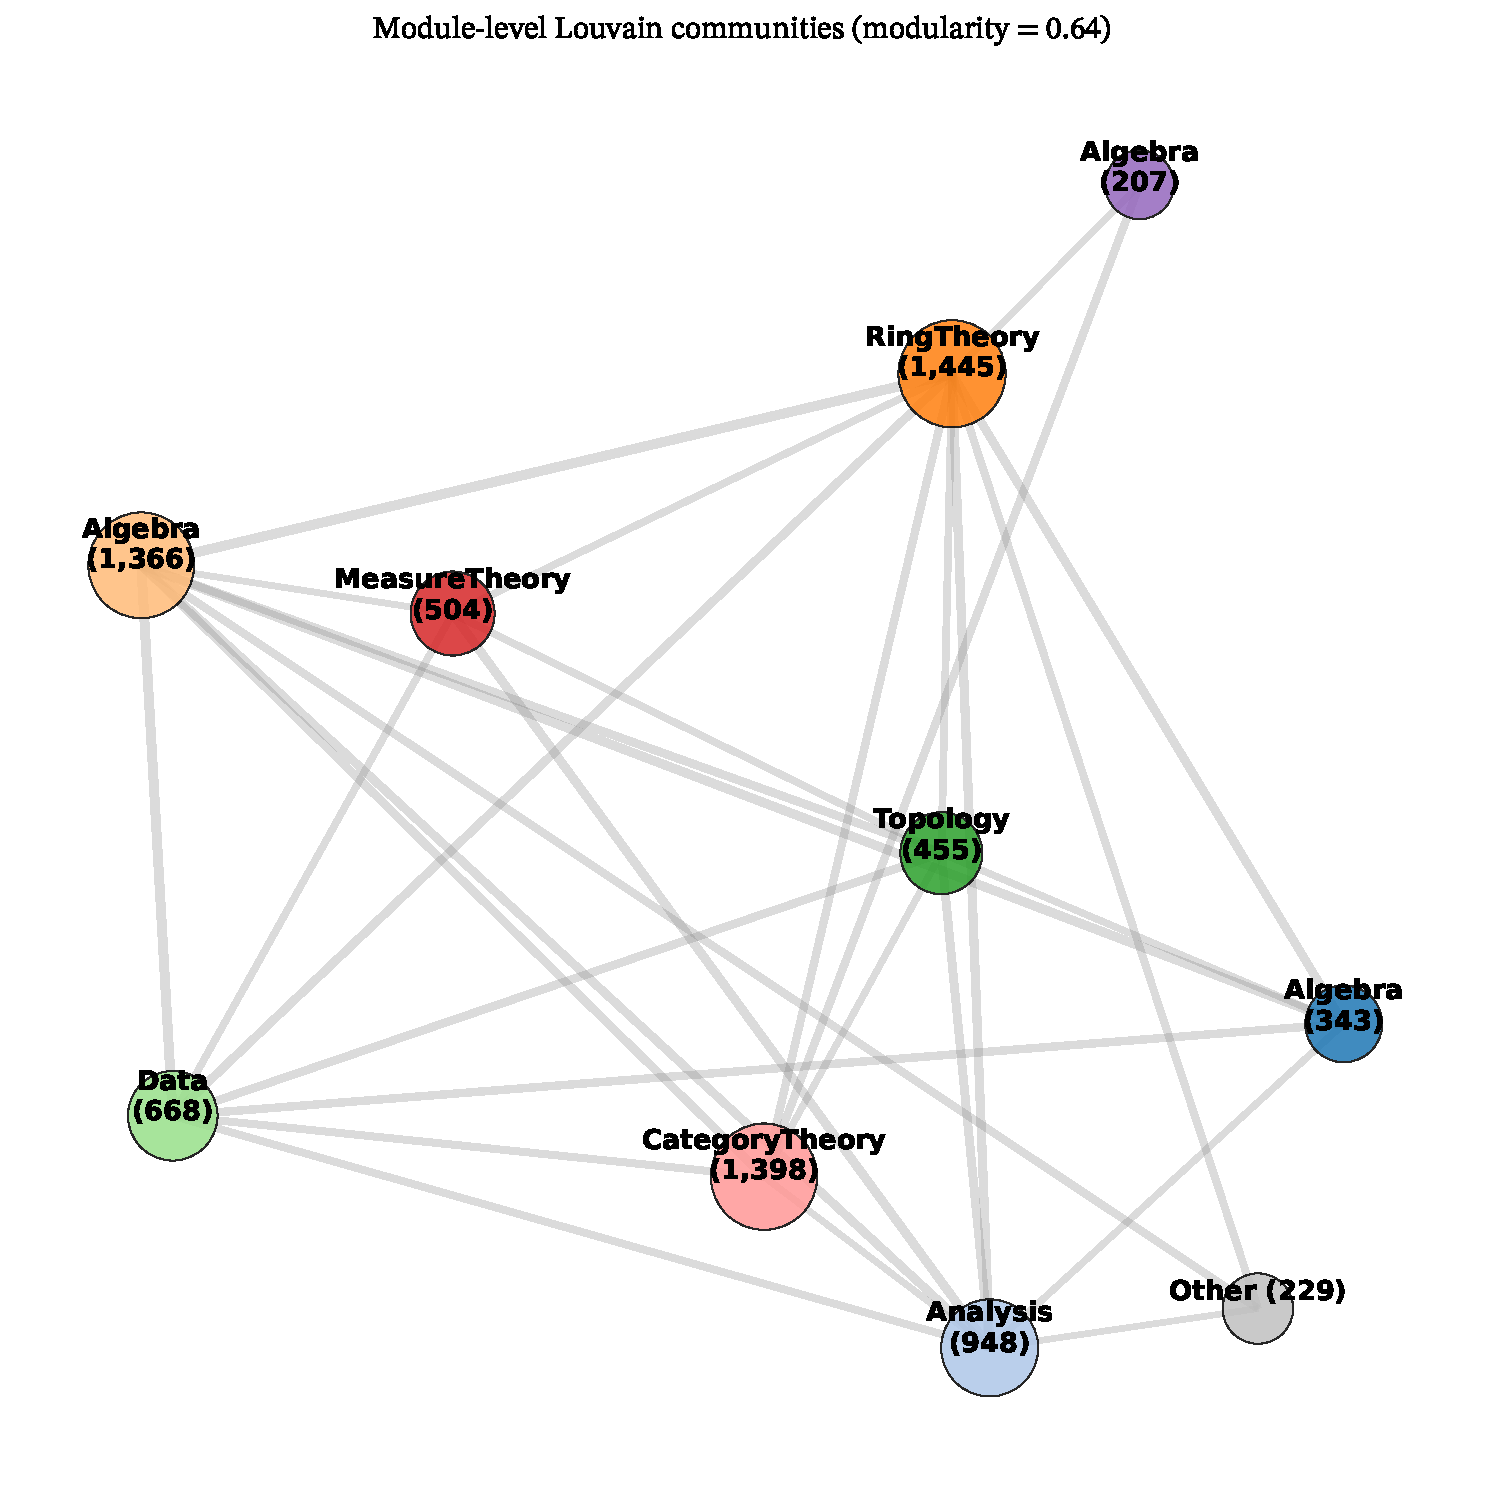
\includegraphics[width=\textwidth]{figures/community_module_graph.pdf}
\caption{Louvain community aggregation graph of $G_{\mathrm{module}}$ (modularity~$= 0.64$). Each node is a community; size $\propto \sqrt{\text{members}}$; labels show the dominant directory and count.}
\label{fig:community-module-graph}
\end{figure}

\begin{figure}[H]
\centering
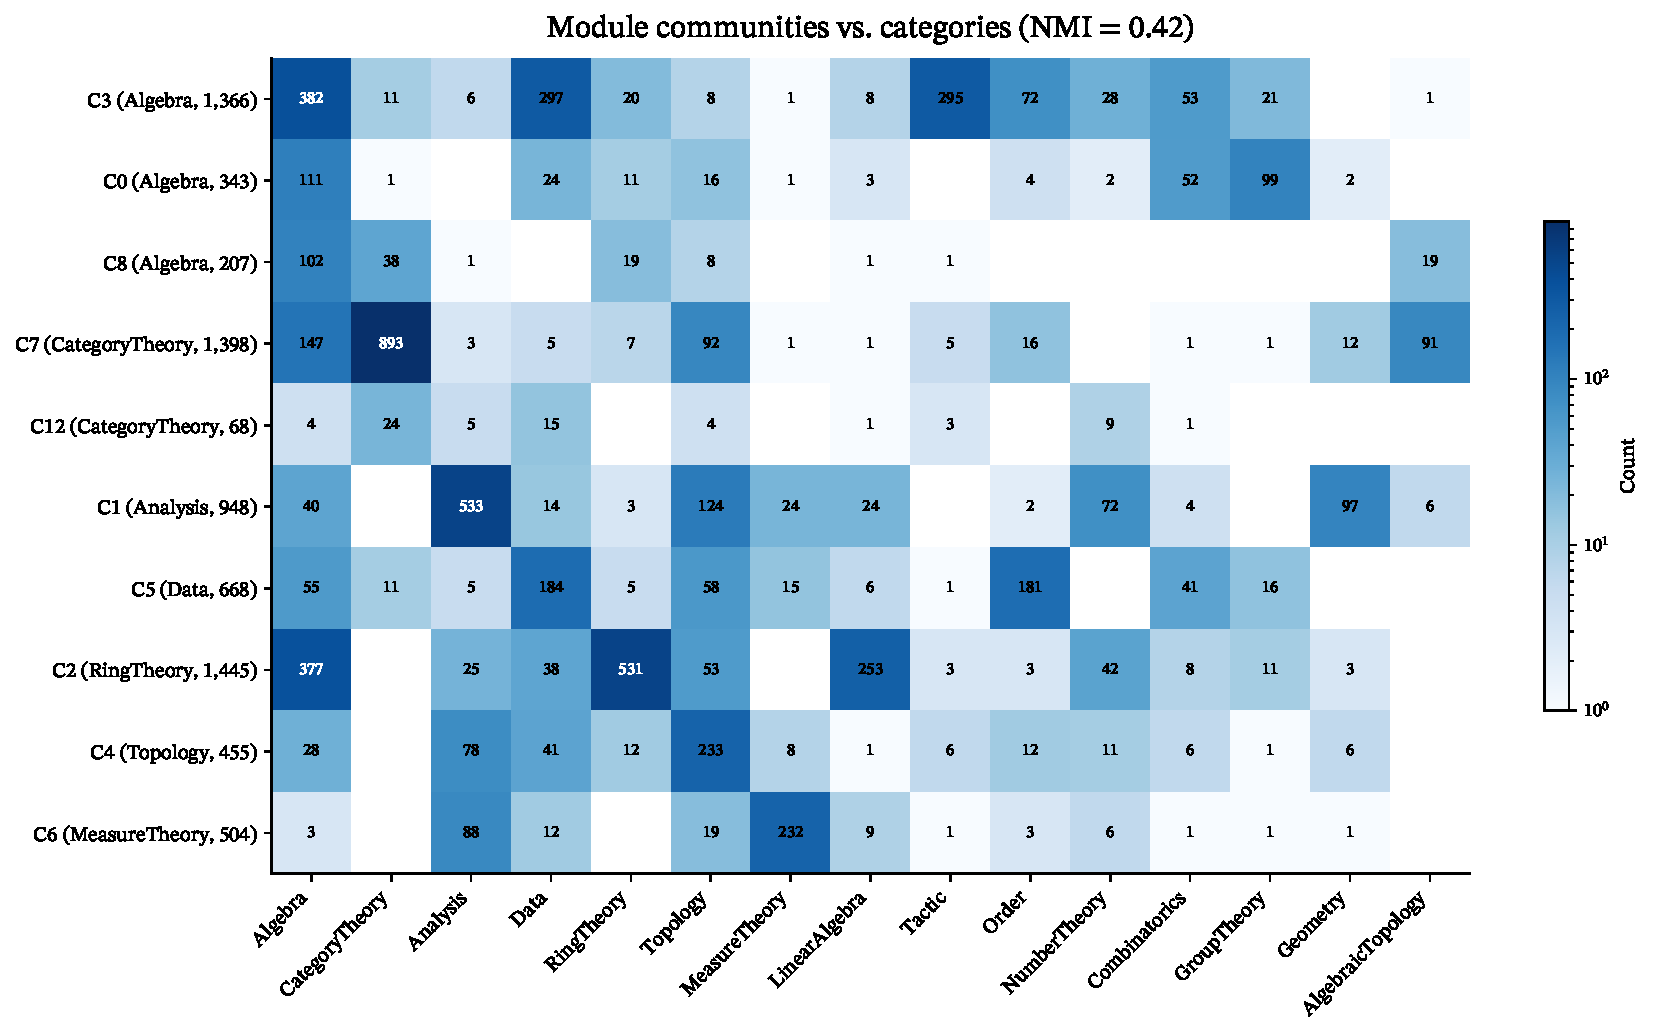
\includegraphics[width=\textwidth]{figures/community_module_heatmap.pdf}
\caption{Community$\,\times\,$directory membership heatmap for $G_{\mathrm{module}}$ (NMI~$= 0.42$, log scale). \module{CategoryTheory} (C7) concentrates sharply in one column; \module{Algebra} fragments across three communities (C3, C0, C8).}
\label{fig:community-module-heatmap}
\end{figure}

\subsubsection{Robustness}
\label{sec:robustness}
\label{sec:sa-robustness}

$G_{\mathrm{module}}$ is weakly connected: all $7{,}563$ modules belong to a single weakly connected component. We assess robustness by measuring the impact of targeted node removal.

\begin{table}[H]
\centering
\caption{Effect of removing the top-5 modules (by in-degree or betweenness) on the number of weakly connected components.}
\label{tab:robustness}
\begin{tabular}{lrr}
\toprule
Removal strategy & \multicolumn{1}{c}{$G_{\mathrm{module}}$} & \multicolumn{1}{c}{$G_{\mathrm{module}}^{-}$} \\
\midrule
None (baseline)          & $1$  & $1$  \\
Top-5 by in-degree       & $29$ & $56$ \\
Top-5 by betweenness     & $20$ & $48$ \\
\bottomrule
\end{tabular}
\end{table}

Removing the five highest in-degree modules (\module{Init}, \module{Tactic.Common}, \module{Analysis.Normed.Group.Basic}, \module{Util.CompileInductive}, and \module{Algebra.Ring.Defs}) fragments the raw graph into $29$ components, though the largest component still contains $7{,}530$ of the original $7{,}563$ nodes. The effect is more pronounced on $G_{\mathrm{module}}^{-}$ ($56$ components), since transitive reduction removes the alternative paths that would otherwise keep the graph connected.

\noindent\textbf{Note.}
\label{rem:robustness}
The fragmentation is modest: even after targeted removal, over $99\%$ of modules remain in the giant component. This resilience stems from the high density of the module graph---each module has, on average, $3.12$ imports, providing redundant connectivity. The transitive reduction is more fragile precisely because it removes this redundancy.
This finding reframes the cognitive redundancy of \S\ref{sec:transitive-reduction}: the edges that developers add for navigability---guided by the categories of~$T$---simultaneously serve as structural insurance, providing alternative paths that keep the network connected when bridges fail.\oliver{SHAKE: ``cognitive redundancy'' and ``navigability'' should be reframed as ``development-ergonomic redundancy'' and ``ease of extension.''}

\begin{figure}[ht]
\centering

\includegraphics[width=0.85\textwidth]{figures/module_robustness_curve.pdf}
\caption{Robustness curves for $G_{\mathrm{module}}$: fraction of nodes in the largest WCC as a function of the fraction removed, under random removal (blue) and targeted removal by PageRank (coral).}
\label{fig:module-robustness}
\end{figure}

Figure~\ref{fig:module-robustness} shows the progressive removal curves. Under random removal, the giant component degrades gracefully---removing $20\%$ of modules leaves $80\%$ connected. Under targeted attack on the highest-PageRank modules, the same $20\%$ removal reduces the giant component to $58\%$, a $22$-percentage-point gap that grows with the removal fraction. The curve confirms the hub-dominated vulnerability signature: the module graph's resilience depends on a small number of high-centrality hubs whose removal fragments the network far more effectively than chance would predict.
